\documentclass[12pt]{article}
\usepackage{listings}
\usepackage{color}
\usepackage{float}
\usepackage{graphicx}

\definecolor{mygreen}{rgb}{0,0.6,0}
\definecolor{mygray}{rgb}{0.5,0.5,0.5}
\definecolor{mymauve}{rgb}{0.58,0,0.82}

\lstset{ %
	xleftmargin=2em,
	backgroundcolor=\color{white},   % choose the background color; you must add \usepackage{color} or \usepackage{xcolor}
	basicstyle=\small,%\footnotesize,        % the size of the fonts that are used for the code
	breakatwhitespace=false,         % sets if automatic breaks should only happen at whitespace
	breaklines=false,                 % sets automatic line breaking
	captionpos=b,                    % sets the caption-position to bottom
	commentstyle=\color{mygreen},    % comment style
	deletekeywords={...},            % if you want to delete keywords from the given language
	escapeinside={\%*}{*)},          % if you want to add LaTeX within your code
	extendedchars=true,              % lets you use non-ASCII characters; for 8-bits encodings only, does not work with UTF-8
	%	frame=single,                    % adds a frame around the code
	keepspaces=true,                 % keeps spaces in text, useful for keeping indentation of code (possibly needs columns=flexible)
	keywordstyle=\color{blue},       % keyword style
	language=VHDL, % the language of the code
	morekeywords={*,...},            % if you want to add more keywords to the set
	numbers=left,                    % where to put the line-numbers; possible values are (none, left, right)
	numbersep=5pt,                   % how far the line-numbers are from the code
	numberstyle=\small\color{mygray}, % the style that is used for the line-numbers
	rulecolor=\color{black},         % if not set, the frame-color may be changed on line-breaks within not-black text (e.g. comments (green here))
	showspaces=false,                % show spaces everywhere adding particular underscores; it overrides 'showstringspaces'
	showstringspaces=false,          % underline spaces within strings only
	showtabs=false,                  % show tabs within strings adding particular underscores
	stepnumber=1,                    % step between two line-numbers. If it's 1, each line will be numbered
	stringstyle=\color{mymauve},     % string literal style
	tabsize=2                  % sets default tabsize to 2 spac                  % show the filename of files included with \lstinputlisting; also try caption instead of title
}
%opening
\title{Project 2: Designing an 8-bit ALU}
\author{Adam Sumner - A20283081 \\ Contribution - 100\% \\ ~\\ ECE 485}
\date{November 16\textsuperscript{th}, 2015}

\begin{document}

\maketitle

\section{Introduction}
The purpose of this project is to implement an 8-bit ALU in the VHDL hardware-description language. The ALU should be able to perform the following functions:
\begin{itemize}
	\item ADD
	\item SUBTRACT
	\item LESS-THAN
	\item AND
	\item NOT
	\item XOR
	\item Bit Shift Left
	\item Arithmetic Bit Shift Right
\end{itemize}
\section{Design}
\subsection{Architecture}
The architecture of the ALU is simple. First and foremost, a \texttt{clk} signal is included. This is necessary because during the design process, it was concluded that all operations will be performed and outputted on the positive edge of the \texttt{clk}. Also, as per the design specification, two inputs \texttt{a} and \texttt{b} must be included. These are both signed vectors of 8 bits because this ALU is designed for 8 bit operations. They are signed because operations like addition and subtraction are included in the ALU's capability. Because in the real world negative numbers are often part of computer programs, it was necessary to make sure that the functionality of the ALU would be able to handle them. Due to the fact that signed numbers are being used, two status bits are included. These are \texttt{ov} and \texttt{zero}. \texttt{ov} is the overflow bit that is set when an overflow/underflow occurs, and \texttt{zero} is the zero status bit that is set when the output is zero. \texttt{op} is the operation bit. This signal is used to select the operation of the ALU to be performed on inputs \texttt{a} and \texttt{b}. \texttt{s} is a selector bit. Because bit shift left, arithmetic bit shift right, and NOT are included in the functionality of the ALU and the ALU always takes two inputs, this signal is included to select which input to perform the shift or NOT operation on. Last an output must be included in the design of the ALU, and this is done by implementing an output \texttt{y} of 8 bits. A visual overview of the ALU is shown in Figure \ref{fig:high-level-overview}.

\begin{figure}[H]
\centering
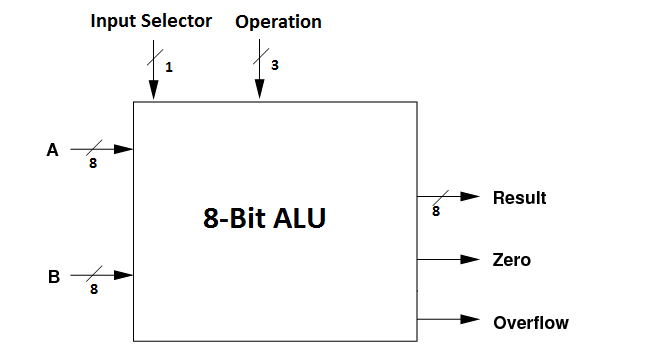
\includegraphics[width=0.7\linewidth]{high-level-overview}
\caption{High Level Overview of Architecture}
\label{fig:high-level-overview}
\end{figure}

\subsection{Behavior}
The behavior section of the code in Section \ref{sec:code} is at its core a switch case on the operation to be performed. Two bit vectors are first declared, \texttt{temp9} and \texttt{temp}. \texttt{temp9} is used in the calculation for overflow and underflow and \texttt{temp} is a temporary storage location of the result so that before its value is outputted from the ALU, its value can be checked for zero to see if the zero status bit should be set or not. A process is defined for the \texttt{clk} signal. If the \texttt{clk} is at its rising edge, then an operation can be performed. The value of the operation to be performed is then assessed. The bit pattern-operation pairs are shown in Table \ref{tab:operations}. When an operation is performed, \texttt{temp} receives the value. 

\begin{table}[H]
	\centering
	\begin{tabular}{|c|c|}
		\hline
		$\texttt{op}_2$$\texttt{op}_1$$\texttt{op}_0$ & \texttt{y} (output) \\ 
		\hline
		000 & bit-wise AND of a and b\\
		\hline
		001 & bit-wise NOT of a and b\\
		\hline
		010 & ADD (a+b) \\
		\hline
		011 & Less Than\\
		\hline
		100 & Subtract (a-b)\\
		\hline
		101 & bit-wise XOR of a and b\\
		\hline
		110 & Logical left shift by one \\
		\hline
		111 & Arithmetic right shift by one bit \\
		\hline
		
	\end{tabular}
	\caption{ALU Operation Description}
	\label{tab:operations}
\end{table}

\noindent AND and XOR are both straightforward operations that do not require any conditionals or overflow checking. NOT involves setting the selector bit to determine which input to perform the NOT operation on. This is done with a simple conditional where if \texttt{s} == 1 then \texttt{a} is complemented and if \texttt{s} == 0, then \texttt{b} is complemented. Addition and subtraction require a little more involvement. First the 8 bit signed vectors \texttt{a} and \texttt{b} are sign extended into 9 bit signed vectors and then added or subtracted and the result is stored in \texttt{temp9}. If the MSB or 9\textsuperscript{th} bit of \texttt{temp9} differs from the 8\textsuperscript{th} bit, then an overflow occurred in the case of addition, and an underflow occurred in the case of subtraction. The \texttt{ov} bit is then set accordingly. The result of \texttt{temp9} is then resized back to 8 bits into \texttt{temp} because the value must still be outputted by the ALU. For the Less Than operation, \texttt{a} is tested if it is less than \texttt{b}. If it is, then the value is set to $11111111_2$, or -1 in decimal. In some old languages, such as Forth, -1 is denoted as the True value for a boolean. If \texttt{a} is not less than \texttt{b}, then temp is set to $00000000_2$, which corresponds to the value of False in most languages. After the switch case is exited, the \texttt{zero} bit is set accordingly, where a 1 denotes False, and a 0 denotes True. The designer of the Assembly Language to correspond with this ALU design may use either the output values -1/0, or the zero status bit to determine the value of the conditional operation. The bit shift operations involve the use of the function \texttt{SHIFT\_LEFT} and \texttt{SHIFT\_RIGHT}. Because an arithmetic shift left and a logical shift left perform the same functionality, an unsigned or signed vector can be fed to the function without worry if the output will differ. However, an arithmetic right shift is used for signed numbers, while a logical right shift is used for unsigned numbers. Luckily, the function \texttt{SHIFT\_RIGHT} has the ability to be overloaded, so depending on the type of vector that is passed in, it will perform the corresponding shift. Since in this case a signed vector is passed in, the function automatically performs an arithmetic shift right. Also, there is a conditional check on the bit selector signal in both shifts. If it is set to 1, then input \texttt{a} is shifted by one bit. If it is set to 0, then input \texttt{b} is shifted by one bit. Because outputs cannot be read if not using a VHDL compiler post 2008, the \texttt{temp} value is used in the conditional at the end of the switch case to determine the \texttt{zero} status bit value. Once established, the value of temp is then written to the output \texttt{y}. Figure \ref{fig:block-dia} shows a more in depth block diagram of what the ALU looks like.
\begin{figure}[H]
\centering
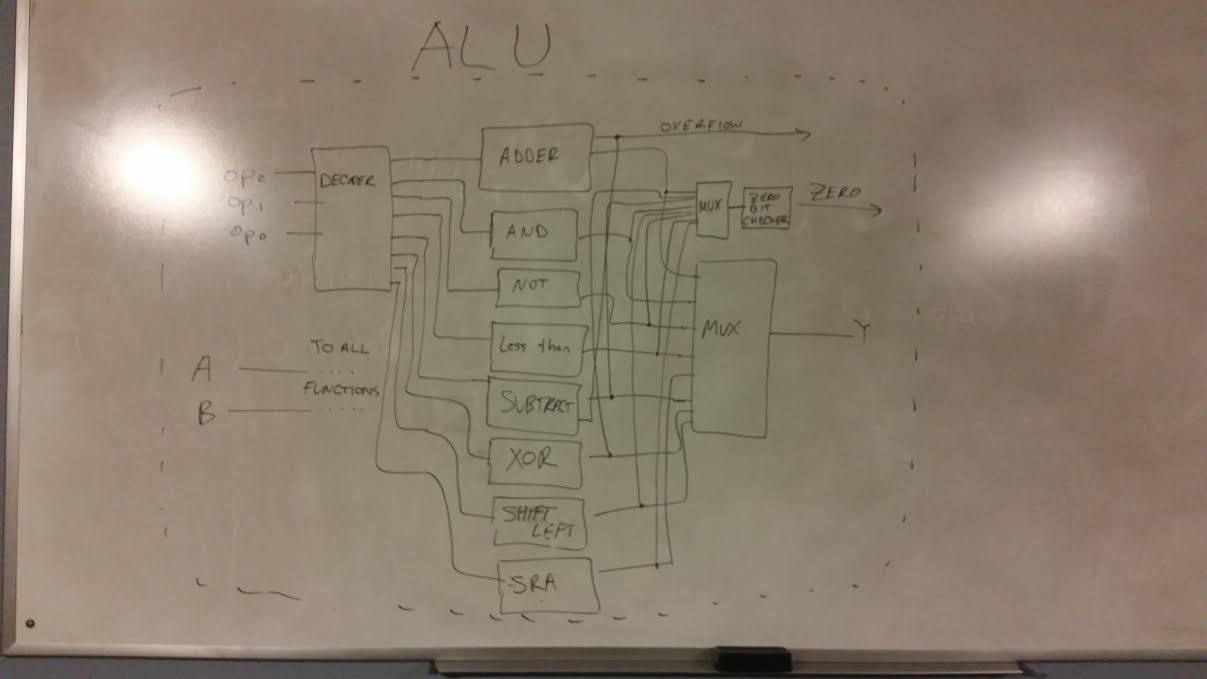
\includegraphics[width=1\linewidth]{block-dia}
\caption{Block Diagram of ALU}
\label{fig:block-dia}
\end{figure}

\subsection{Code}\label{sec:code}
\lstset{language=VHDL}
\lstinputlisting{../alu.vhd}
\begin{lstlisting}

\end{lstlisting}

\section{Analysis}
While the specification of the ALU to be implemented was not specific, the goal of the design was to give the ALU the basic defined functionality with added features. For example, the design simply said to include operations such as addition and subtraction, while the implemented design included signed addition and subtraction with the ability to detect overflow/underflow or if the value is zero using status bits. While this increased the complexity of the logic of the design, it enables the ALU to be a unit that can actually be utilized rather than a unit that ``just gets the bare minimum job done". A downfall to this decision however is the range of numbers that can be calculated. 1 bit is lost due to the sacrifice for a sign bit, but this sacrifice is necessary if the ALU is to work in conjunction with any modern program. To improve upon the design however, a carry bit should be implemented. This would mean that the ALU would support unsigned addition and subtraction as well as signed. An ALU in practice does not know whether it is performing signed or unsigned operations, it just sets the status bits accordingly. The carry bit would be an easy addition to the current design by just checking if the MSB of \texttt{temp9} is set to 1 . Furthermore, more operations could be included in the design. OR, NAND, NOR, etc. could be included in the list of supported operations, as well as multiplication and division. The logic gates would be easy to implement, while multiplication and division would change the size of the output vector to be 16 bits. The current state of the design allows these additional functions to be easily implemented in the future. As more functionality is added, more hardware will be needed. Thanks to Moore's law, hardware is quite cheap to implement, so adding more hardware to the 8 bit ALU would not cost much to the manufacturer.
\section{Simulation Results}
This section will walk through each operation that the ALU is capable of performing. A Clock cycle of 10ns was used for the simulation. Figure \ref{fig:and} shows the results of anding $F1_{16}$ with $82_{16}$. The proper output $80_{16}$ is displayed as well as the proper value of the zero status bit. 


\begin{figure}[H]
\centering
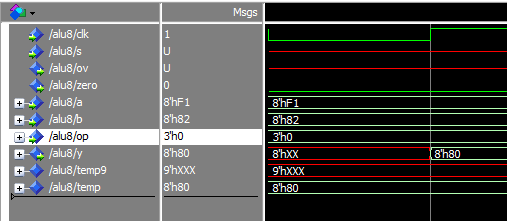
\includegraphics[width=1\linewidth]{and}
\caption{Result of AND}
\label{fig:and}
\end{figure}

Figure \ref{fig:not-a} shows the result of selecting the input a to be negated. Input a has the value of $F1_{16}$ and the correct output of $0E_{16}$ is calculated. The zero bit is also correctly set.

\begin{figure}[H]
\centering
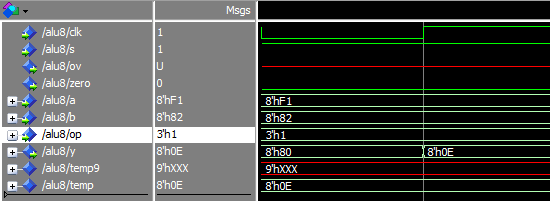
\includegraphics[width=1\linewidth]{not-a}
\caption{Result of NOT with input a}
\label{fig:not-a}
\end{figure}

Figure \ref{fig:not-b} shows the result of selecting the input a to be negated. Input a has the value of $82_{16}$ and the correct output of $7D_{16}$ is calculated. The zero bit is also correctly set.
\begin{figure}[H]
\centering
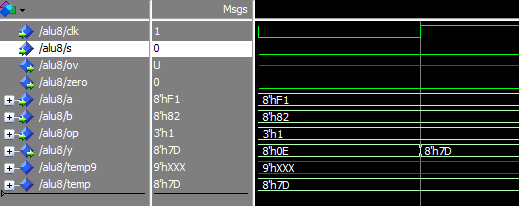
\includegraphics[width=1\linewidth]{not-b}
\caption{Result of NOT with input b}
\label{fig:not-b}
\end{figure}

Figure \ref{fig:addition} shows the result of adding $F1_{16}$ and $82_{16}$. The correct output of $73_{16}$ is shown and the overflow bit is in fact set to one. This is because two negative numbers produced a positive number! The zero bit is also set correctly.

\begin{figure}[H]
\centering
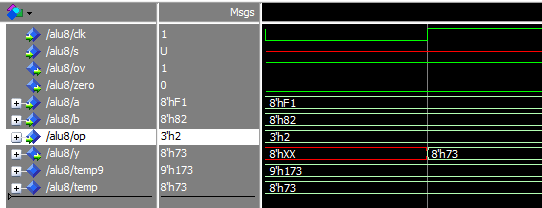
\includegraphics[width=1\linewidth]{addition}
\caption{Result of Addition}
\label{fig:addition}
\end{figure}

Figure \ref{fig:addition-no-overflow} shows the result of adding $08_{16}$ and $08_{16}$. The correct output of $10_{16}$ is shown. Both status bits are set correctly.

\begin{figure}[H]
\centering
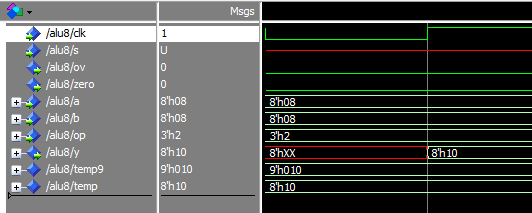
\includegraphics[width=1\linewidth]{addition-no-overflow}
\caption{Addition Without Overflow}
\label{fig:addition-no-overflow}
\end{figure}

Figure \ref{fig:less-than} shows the result of checking if $00_{16}$ is less than $08_{16}$. The output is $FF_{16}$ and the zero bit is set to 0 which is the expected result.

\begin{figure}[H]
\centering
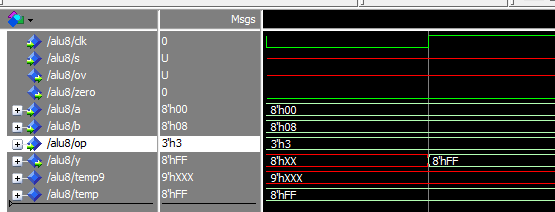
\includegraphics[width=1\linewidth]{less-than}
\caption{Result of Less Than}
\label{fig:less-than}
\end{figure}

Figure \ref{fig:subtract} shows the result of $07_{16} - 02_{16}$. The expected result $05_{16}$ is outputted and the overflow and zero status bits are both set correctly to 0.

\begin{figure}[H]
\centering
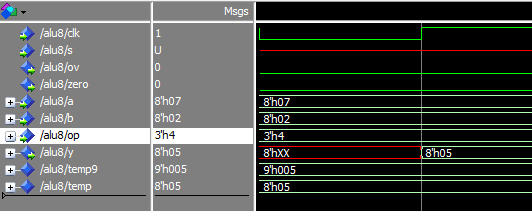
\includegraphics[width=1\linewidth]{subtract}
\caption{Result of Subtract}
\label{fig:subtract}
\end{figure}

Figure \ref{fig:XOR} shows the result of $E6_{16} \oplus E8_{16}$. The correct result of $0E_{16}$ is outputted.

\begin{figure}[H]
\centering
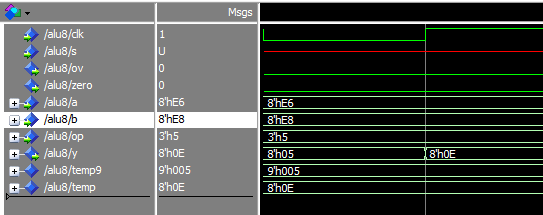
\includegraphics[width=1\linewidth]{XOR}
\caption{Result of XOR}
\label{fig:XOR}
\end{figure}

Figure \ref{fig:sll-a} shows the result of shifting input \texttt{a} with a value of $E6_{16}$ left by 1 bit. The correct output is displayed as $CC_{16}$.
\begin{figure}[H]
\centering
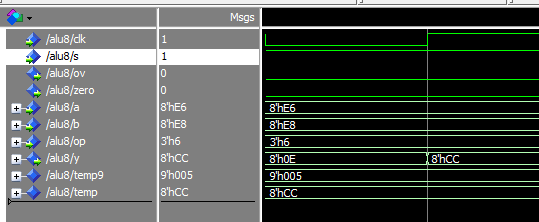
\includegraphics[width=1\linewidth]{sll-a}
\caption{Shift Left on Input \texttt{a}}
\label{fig:sll-a}
\end{figure}

Figure \ref{fig:sll-b} shows the result of shifting input \texttt{b} with a value of $E8_{16}$ left by 1 bit. The correct output is displayed as $D0_{16}$.

\begin{figure}[H]
\centering
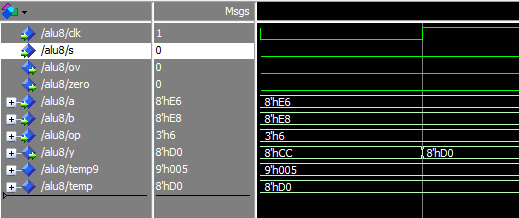
\includegraphics[width=1\linewidth]{sll-b}
\caption{Shift Left on Input \texttt{b}}
\label{fig:sll-b}
\end{figure}

Figure \ref{fig:sra-a} shows the result of arithmetically shifting input \texttt{a} with a value of $E6_{16}$ right by 1 bit. The correct result of $F3_{16}$ is outputted.
\begin{figure}[H]
\centering
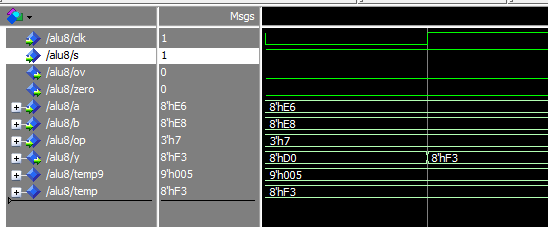
\includegraphics[width=1\linewidth]{sra-a}
\caption{Arithmetic Shift Right on Input \texttt{a}}
\label{fig:sra-a}
\end{figure}


Figure \ref{fig:sra-b} shows the result of arithmetically shifting input \texttt{b} with a value of $E8_{16}$ right by 1 bit. The correct result of $F4_{16}$ is outputted.

\begin{figure}[H]
\centering
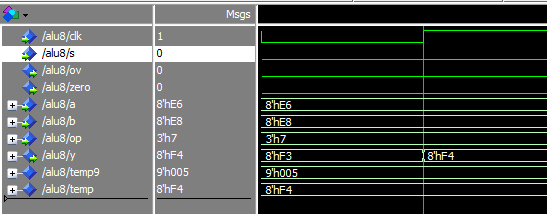
\includegraphics[width=1\linewidth]{sra-b}
\caption{Arithmetic Shift Right on Input \texttt{b}}
\label{fig:sra-b}
\end{figure}


On average, each operation took around 2-3 clock cycles to display output which shows the efficiency of the designed ALU.
\section{Conclusion}
The design and implementation of an 8-bit ALU was a success. An architecture was designed and a behavior was successfully put into practice. All requested functionality was achieved with added on features. This 8-bit ALU can now be used in further projects.
\end{document}
